% Hub architecture (Chapter 3). Shapes from configs/v6_3.yaml and src/v3/bridge.py of the research repo.
\usetikzlibrary{positioning,arrows.meta,fit}
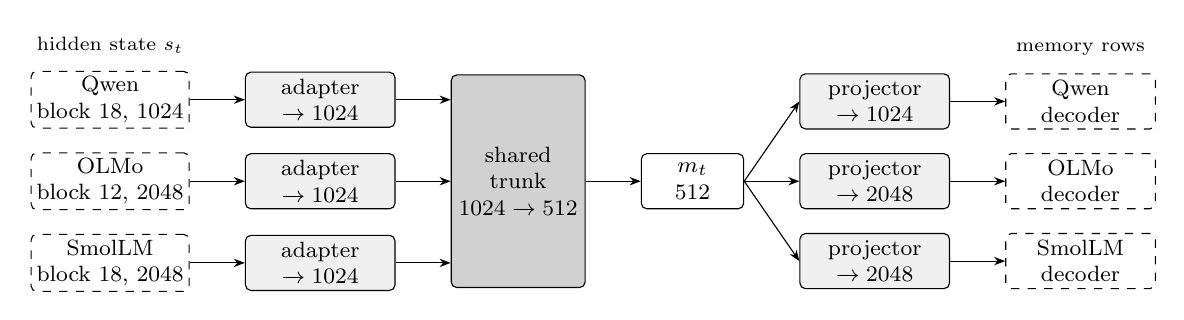
\begin{tikzpicture}[
  font=\footnotesize, >={Stealth[length=4pt]},
  box/.style={draw, rounded corners=2pt, minimum height=7mm, minimum width=19mm, align=center, inner sep=2pt},
  own/.style={box, fill=black!6},
  shared/.style={box, fill=black!18, minimum height=27mm, minimum width=17mm},
  frozen/.style={box, dashed},
  node distance=3mm and 7mm]
  \node[frozen] (sq) {Qwen\\block 18, 1024};
  \node[frozen, below=of sq] (so) {OLMo\\block 12, 2048};
  \node[frozen, below=of so] (ss) {SmolLM\\block 18, 2048};
  \node[own, right=of sq] (aq) {adapter\\$\to 1024$};
  \node[own, right=of so] (ao) {adapter\\$\to 1024$};
  \node[own, right=of ss] (as) {adapter\\$\to 1024$};
  \node[shared, right=of ao] (tr) {shared\\trunk\\$1024 \to 512$};
  \node[box, right=of tr, minimum width=13mm] (m) {$m_t$\\512};
  \node[own, right=of m] (po) {projector\\$\to 2048$};
  \node[own, above=of po] (pq) {projector\\$\to 1024$};
  \node[own, below=of po] (ps) {projector\\$\to 2048$};
  \node[frozen, right=of pq] (dq) {Qwen\\decoder};
  \node[frozen, right=of po] (do) {OLMo\\decoder};
  \node[frozen, right=of ps] (ds) {SmolLM\\decoder};
  \foreach \a/\b in {sq/aq, so/ao, ss/as, pq/dq, po/do, ps/ds} \draw[->] (\a) -- (\b);
  \draw[->] (aq.east) -- (tr.west |- aq.east);
  \draw[->] (ao.east) -- (tr.west);
  \draw[->] (as.east) -- (tr.west |- as.east);
  \draw[->] (tr) -- (m);
  \draw[->] (m.east) -- (pq.west);
  \draw[->] (m.east) -- (po.west);
  \draw[->] (m.east) -- (ps.west);
  \node[above=1mm of sq, font=\scriptsize] {hidden state $s_t$};
  \node[above=1mm of dq, font=\scriptsize] {memory rows};
\end{tikzpicture}
